

%%%%%%%%%%%%%%%%%%%%%%%%%%%%%%%%%%%

\begin{frame}
\frametitle{Filtros FIR con $h(n)$ real y $H(e^{jw})$ de fase lineal I}

\vspace{-0.2cm}



\begin{itemize}
\footnotesize
\item Un filtro FIR con respuesta en frecuencia de fase lineal cumple que:
\begin{itemize}
\footnotesize
\item $H(e^{jw})=\sum_{n=0}^N h(n)e^{-jwn}=e^{j(\alpha w + \beta)} \hat H(e^{jw})$, con $\hat H(e^{jw})$ respuesta fase cero (respuesta en amplitud ($\pm$) vs. desfase).
\end{itemize}

\visible<2->{

\item Un filtro FIR con $h(n)$ real cumple que:

\begin{itemize}
\footnotesize
\item {$H^*(e^{jw})=H(e^{-jw})$}  \visible<3->{ $\rightarrow$ \alert{$\hat H(e^{jw})e^{j(\alpha w+\beta)}=\hat H(e^{-jw})e^{-j(\alpha(-w)+\beta)}$  (*)}}

\item El módulo de la respuesta en frecuencia es una función par: $|H(e^{jw})|=|H(e^{-jw})|$  \visible<4->{$\rightarrow$ \alert{ $\hat H(e^{jw})= \pm \hat H(e^{-jw})$}}

\end{itemize}

}

\visible<5->{\item Si  \alert{$\hat H(e^{jw})=+ \hat H(e^{-jw})$}}  \visible<10->{\alert{$\rightarrow h(n)=h(N-n)$} y \alert{$H(e^{jw})=\pm e^{-j\frac{N}{2}w}\hat H(e^{jw})$}}

\color{gray}
{\scriptsize
\visible<6->{

(*) $\rightarrow e^{j(\alpha w+\beta)}\!=\!e^{j(\alpha w-\beta)} \rightarrow e^{j\beta}\!=\!e^{-j\beta} $ $\rightarrow \beta\!=\!k\pi$}

\visible<7->{

$H(e^{jw})=e^{j(\alpha w + \beta)} \hat H(e^{jw}) \rightarrow  \hat H(e^{jw})=\pm e^{-j\alpha w} H(e^{jw})=\pm\sum_{n=0}^{N} h(n) e^{-jw(n+\alpha)} $}

\visible<8->{

\alert{$\hat H(e^{jw})=\pm\sum_{n=0}^{N} h(n) e^{-jw(n+\alpha)}$  }}

\visible<9->{
$\hat H(e^{-jw})=\pm\sum_{l=0}^{N} h(l) e^{jw(l+\alpha)}=\pm\sum_{n=N}^{0} h(N-n) e^{jw(N-n+\alpha)}$
}

\visible<10->{
$\sum_{n=0}^{N} h(n) e^{-jw(n+\alpha)}\!=\!\sum_{n=N}^{0} h(N-n) e^{jw(N-n+\alpha)}  \rightarrow \alpha\!=\!-N/2\:$ y $\:h(n)\!=\!h(N\!-\!n)$}
}

\color{black}
\visible<5->{\item Si \alert{$\hat H(e^{jw})=- \hat H(e^{-jw})$}} \visible<11->{\alert{$\rightarrow h(n)=-h(N-n)$} y \alert{$H(e^{jw})= e^{-j(\frac{N}{2}w \mp \frac{\pi}{2})}\hat H(e^{jw})$}}


\color{gray}

\visible<11->{

{\scriptsize
(*) $\rightarrow e^{j(\alpha w+\beta)}\!=\!-e^{j(\alpha w-\beta)} \rightarrow e^{j\beta}\!=-\!e^{-j\beta} $ $\rightarrow \beta=\frac{\pi}{2} \:\:$ o $\:\:\beta=\frac{3\pi}{2}$ 

$H(e^{jw})=e^{j(\alpha w + \beta)} \hat H(e^{jw}) \rightarrow  \hat H(e^{jw})=\mp  j e^{-j\alpha w} H(e^{jw})=\mp j\sum_{n=0}^{N} h(n) e^{-jw(n+\alpha)} $

\alert{$\hat H(e^{jw})=\mp j \sum_{n=0}^{N} h(n) e^{-jw(n+\alpha)}$  }

$\hat H(e^{-jw})=\mp j \sum_{l=0}^{N} h(l) e^{jw(l+\alpha)}=\mp j \sum_{n=N}^{0} h(N-n) e^{jw(N-n+\alpha)}$

$\sum_{n=0}^{N} h(n) e^{-jw(n+\alpha)}\!=\!-\!\sum_{n=0}^{N} h(N-n) e^{jw(N-n+\alpha)}  \rightarrow \alpha\!=\!-N/2$ y $h(n)\!=\!-h(N\!-\!n)$
}
}
\end{itemize}
\end{frame}

%%%%%%%%%%%%

\begin{frame}
\frametitle{Filtros FIR con $h(n)$ real y $H(e^{jw})$ de fase lineal II}
\footnotesize
\begin{itemize}
\item Además de las dos posibilidades de la respuesta de fase cero ($\hat H(e^{jw})=\pm \hat H(e^{-jw})$), N puede ser par o impar. Este hecho hace que existan cuatro tipos de filtro FIR de fase lineal:

\item Si  \alert{$\hat H(e^{jw})=+ \hat H(e^{-jw})$}  \alert{$\rightarrow h(n)=h(N-n)$}, \alert{$H(e^{jw})=\pm e^{-j\frac{N}{2}w}\hat H(e^{jw})$} y

\hspace{3.5cm} \alert{$\hat H(e^{jw})=\pm\sum_{n=0}^{N} h(n) e^{-jw(n-N/2)}$  }

\begin{itemize}
\footnotesize

\visible<2->{

\item Tipo 1: $h(n)=h(N-n)$ con $0\le n \le N$ y N par:

\vspace{0.1cm}
\hspace{1.05cm}$\hat H(e^{jw})=h(N/2)+2\sum_{n=1}^{N/2}h(\frac{N}{2}-n)cos(wn)$

}

\vspace{0.2cm}
\visible<3->{

\item Tipo 2: $h(n)=h(N-n)$ con $0\le n \le N$ y N impar:

\vspace{0.1cm}
\hspace{1.05cm}$\hat H(e^{jw})=2\sum_{n=1}^{(N+1)/2}h(\frac{N+1}{2}-n)cos(w(n-1/2))$
}
\end{itemize}

\item Si \alert{$\hat H(e^{jw})=- \hat H(e^{-jw})$} \alert{$\rightarrow h(n)=-h(N-n)$}, \alert{$H(e^{jw})= e^{-j(\frac{N}{2}w \mp \frac{\pi}{2})}\hat H(e^{jw})$} y

\hspace{3.5cm} \alert{$\hat H(e^{jw})=\mp j \sum_{n=0}^{N} h(n) e^{-jw(n-N/2)}$  }


\begin{itemize}
\footnotesize

\visible<4->{

\item Tipo 3: $h(n)=-h(N-n)$ con $0\le n \le N$ y N par:

\vspace{0.1cm}
\hspace{1.05cm}$\hat H(e^{jw})=h(N/2)+2\sum_{n=1}^{N/2}h(\frac{N}{2}-n)sen(wn)$
}

\vspace{0.2cm}

\visible<5->{

\item Tipo 4: $h(n)=-h(N-n)$ con $0\le n \le N$ y N impar:

\vspace{0.1cm}
\hspace{1.05cm}$\hat H(e^{jw})=2\sum_{n=1}^{(N+1)/2}h(\frac{N+1}{2}-n)sen(w(n-1/2))$
}
\end{itemize}
\end{itemize}

\end{frame}

%%%%%%%%%%

\begin{frame}
\frametitle{Filtros FIR con $h(n)$ real y $H(e^{jw})$ de fase lineal III}
\footnotesize
\begin{itemize}
\item Localización de los ceros:
\begin{itemize}
\footnotesize
\item $h(n)$ es real tiene las raíces (ceros) reales o complejas conjugadas

\vspace{0.1cm}

\item Si los filtros son FIR de fase lineal:

\begin{itemize}
\footnotesize
\item $h(n)=h(N-n)$

\vspace{0.1cm}

$H(z)\!=\!\sum_{n=0}^N h(n)z^{-n}\!=\!\sum_{n=0}^N h(N\!-\!n)z^{-n}\!=\!\sum_{m=0}^N h(m)z^{-N\!+\!m}\!=$

\vspace{0.1cm}

\hspace{0.7cm}$=\!z^{-N}H(z^{-1})$


\vspace{0.1cm}

\item $h(n)=-h(N-n)$

\vspace{0.1cm}

$H(z)\!=\!\sum_{n=0}^N \!h(n)z^{-n}\!=\!\!-\!\sum_{n=0}^N \!h(N\!-\!n)z^{-n}\!=\!\!-\!\sum_{m=0}^N \!h(m)z^{-N\!+\!m}\!=$

\vspace{0.1cm}

\hspace{0.7cm}$=\!-z^{-N}H(z^{-1})$

\end{itemize}
\end{itemize}
\item Como $z=re^{j\theta}$ y $z^{-1}=\frac{1}{r}e^{-j\theta}$, los ceros de los FIR de fase lineal representan una simetría especular respecto al círculo unidad.

\item Los cuatro tipos de filtros se diferencian en el número de ceros que hay en +1 y -1.
\begin{itemize}
\scriptsize
\item \alert{Tipo 1 (N par): Un número par o ningún cero en +1 y -1.}
\item \alert{Tipo 2 (N impar): Un número par o ningún cero en +1 y un número impar en -1.}
\item \alert{Tipo 3 (N par): Un número impar en +1 y -1.}
\item \alert{Tipo 4 (N impar): Un número impar +1 y un número par o ninguno en -1.}

\end{itemize}


\end{itemize}

\end{frame}

%%%%%%%%%%%%%%%%%%%%%%%

\begin{frame}
\frametitle{Filtros FIR con $h(n)$ real y $H(e^{jw})$ de fase lineal IV}

\footnotesize

Resumen de las características:

\begin{itemize}

\item Como $z=re^{j\theta}$ y $z^{-1}=\frac{1}{r}e^{-j\theta}$, los ceros de los FIR de fase lineal representan una simetría especular respecto al círculo unidad.

\item $h(n)=h(N-n)$ con $0\le n \le N$,  $\:\:H(e^{jw})=\pm e^{-j\frac{N}{2}w}\hat H(e^{jw})$


\begin{itemize}
\footnotesize
\item Tipo 1: N par, y un número par o ningún cero en +1 y -1

\vspace{0.1cm}

\hspace{1.05cm}$\hat H(e^{jw})=h(N/2)+2\sum_{n=1}^{N/2}h(\frac{N}{2}-n)cos(wn)$



\vspace{0.1cm}

\item Tipo 2: N impar, y un número par o ningún cero en +1 y un número impar en -1.

\vspace{0.1cm}
\hspace{1.05cm}$\hat H(e^{jw})=2\sum_{n=1}^{(N+1)/2}h(\frac{N+1}{2}-n)cos(w(n-1/2))$

\vspace{0.1cm}

\end{itemize}

\item Si $h(n)=-h(N-n)$ con $0\le n \le N$,  $\:\:H(e^{jw})= e^{-j(\frac{N}{2}w \mp \frac{\pi}{2})}\hat H(e^{jw})$

\begin{itemize}
\footnotesize
\item Tipo 3: N par, y un número impar de ceros en +1 y -1

\vspace{0.1cm}
\hspace{1.05cm}$\hat H(e^{jw})=h(N/2)+2\sum_{n=1}^{N/2}h(\frac{N}{2}-n)sen(wn)$

\vspace{0.1cm}


\item Tipo 4: N impar, y un número impar de ceros en +1 y un número par o ninguno en -1

\vspace{0.1cm}
\hspace{1.05cm}$\hat H(e^{jw})=2\sum_{n=1}^{(N+1)/2}h(\frac{N+1}{2}-n)sen(w(n-1/2))$

\end{itemize}
\end{itemize}

\end{frame}

%%%%%%%%%%%%%%%%%%%%%%%

\begin{frame}
\frametitle{Ejemplo de diseño de un filtro FIR de fase lineal}

\footnotesize

\color{olivegreen} Diseñar un FIR tipo 1 de longitud 9  con ceros en -0.5, 0.3+0.5i y $-1/2+\frac{\sqrt{3}}{2}i$

\color{gray}

$z=-0.5  \rightarrow z=-\frac{1}{0.5}$

$z=0.3+0.5i  \rightarrow z=0.3-0.5i, 1/(0.3+0.5i), 1/(0.3-0.5i) $

$z=0.5+\frac{\sqrt{3}}{2}i \rightarrow z=0.5-\frac{\sqrt{3}}{2}i$

\vspace{0.1cm}

Ya tenemos los 8 ceros necesarios para un FIR de longitud 9.

\vspace{0.1cm}

h(n)=[1, -0.8647, 0.2929,6.8276,-7.2641,6.8276,0.2929,-0.8647,1]


\begin{columns}[c]
\begin{column}{4cm}
\lstinputlisting{./Matlab/EjFaseLineal.m}
\end{column}
\begin{column}{7.6cm}
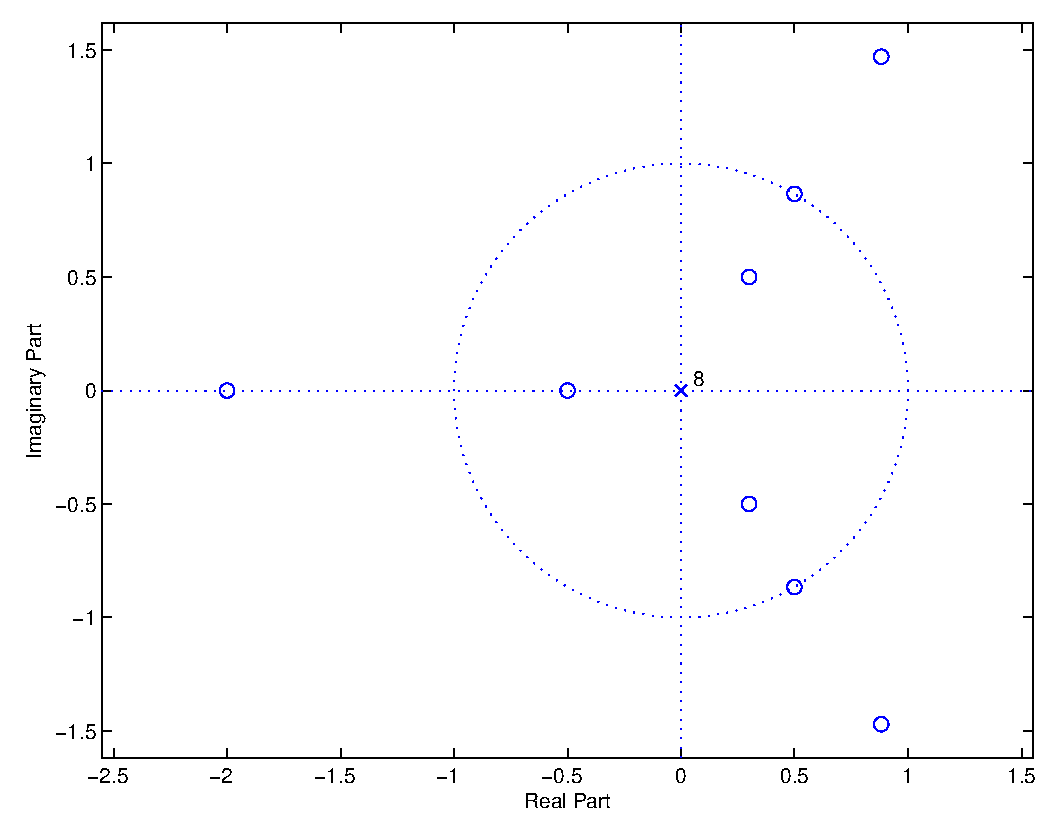
\includegraphics[width=3.8cm]{./Figures/EjFaseLineal1.eps}
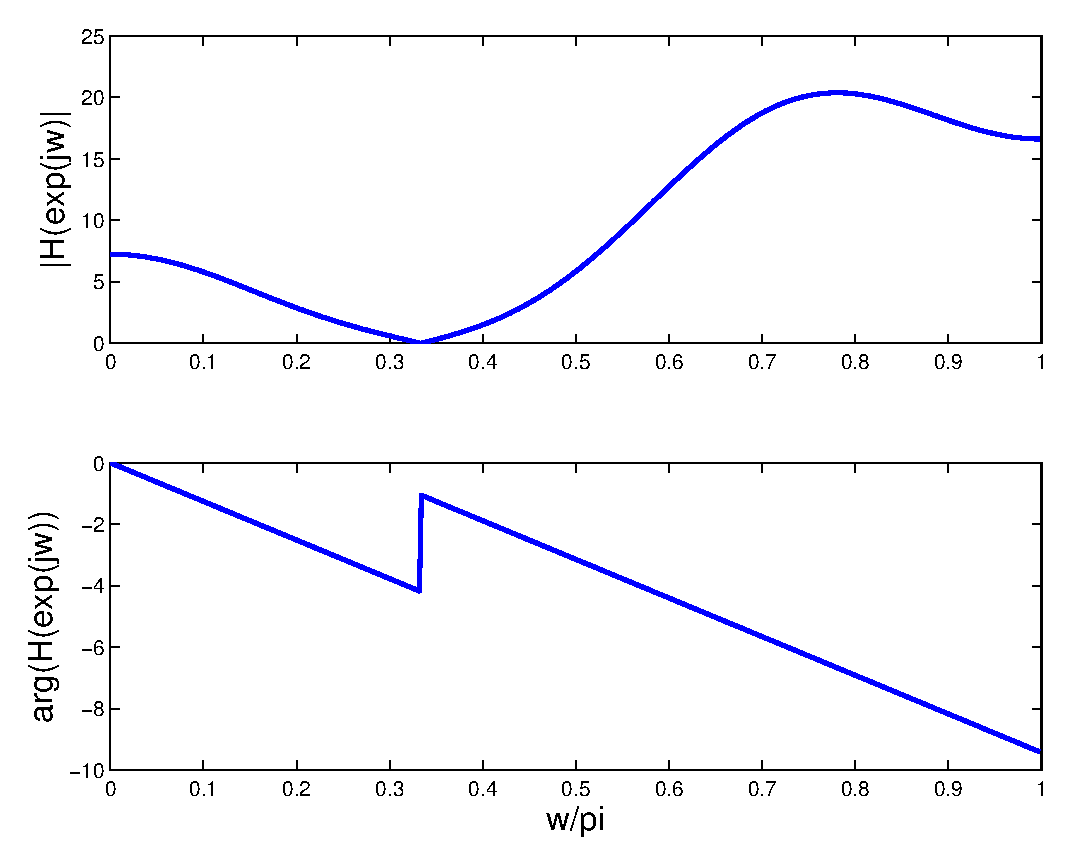
\includegraphics[width=3.8cm]{./Figures/EjFaseLineal2.eps}
\end{column}
\end{columns}





\end{frame}
